\[
    \begin{gathered}
        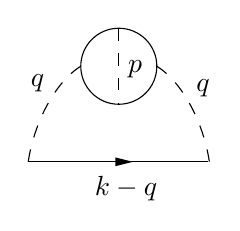
\begin{tikzpicture}[x=0.75pt,y=0.75pt,yscale=-0.7,xscale=0.7]
            %uncomment if require: \path (0,300); %set diagram left start at 0, and has height of 300
            
            %Straight Lines [id:da19683421857457994] 
            \draw    (96,175) -- (219.71,175) ;
            %Straight Lines [id:da2027210917931932] 
            \draw    (168,175.12) ;
            \draw [shift={(168,175.12)}, rotate = 180] [fill={rgb, 255:red, 0; green, 0; blue, 0 }  ][line width=0.08]  [draw opacity=0] (12,-3) -- (0,0) -- (12,3) -- cycle    ;
            %Shape: Circle [id:dp8177746314896752] 
            \draw   (132.17,109.33) .. controls (132.17,94.88) and (143.88,83.17) .. (158.33,83.17) .. controls (172.78,83.17) and (184.5,94.88) .. (184.5,109.33) .. controls (184.5,123.78) and (172.78,135.5) .. (158.33,135.5) .. controls (143.88,135.5) and (132.17,123.78) .. (132.17,109.33) -- cycle ;
            %Curve Lines [id:da8337458763239065] 
            \draw  [dash pattern={on 4.5pt off 4.5pt}]  (96,175) .. controls (100,148.67) and (114,120.67) .. (132.17,109.33) ;
            %Curve Lines [id:da4927523430855625] 
            \draw  [dash pattern={on 4.5pt off 4.5pt}]  (220.67,175) .. controls (216.67,148.67) and (202.67,120.67) .. (184.5,109.33) ;
            %Straight Lines [id:da8574857978112103] 
            \draw  [dash pattern={on 4.5pt off 4.5pt}]  (158.33,83.17) -- (158.33,136.17) ;
            
            % Text Node
            \draw (140,183.08) node [anchor=north west][inner sep=0.75pt]    {$k-q$};
            % Text Node
            \draw (96,113.4) node [anchor=north west][inner sep=0.75pt]    {$q$};
            % Text Node
            \draw (210,116.4) node [anchor=north west][inner sep=0.75pt]    {$q$};
            % Text Node
            \draw (163,103.4) node [anchor=north west][inner sep=0.75pt]    {$p$};          
            \end{tikzpicture}            
    \end{gathered} \quad \sim e^6 \int \dd[3]{\vb*{q}} \frac{1}{q^2} \frac{1}{q^2} \int \dd[3]{\vb*{p}} \frac{1}{p^2} \sim \frac{e^6}{q}
\]